\chapter{Theoretical Background}\label{ch:theoretical-background}

\section{Introduction}\label{sec:introduction}
This chapter reviews existing literature across three interconnected areas: \textbf{Impact Measurement and Management (IMM)}, \textbf{public sector innovation (PSI)}, and the application of \textbf{Artificial Intelligence (AI)} in these domains.
The objective is to establish a conceptual foundation for AI-supported, values-driven impact evaluation in public innovation ecosystems, and to identify gaps that the thesis artefact implemented in \textit{Inluma} will address.

\section{Impact Measurement and Management (IMM)}\label{sec:imm}
The measurement of impact, particularly in social and public sector contexts, has evolved significantly over the past decades.
Scholars such as \textcite{ebrahim2014measuring} emphasize the importance of aligning measurement approaches with a theory of change and organizational strategy.
Organizations often struggle to balance accountability and learning, particularly when the expected impact is diffuse or long-term.

\textcite{nicholls2012measuring} highlight tensions between standardized, quantitative measurement systems and the qualitative, context-specific nature of many social interventions.
Their work formalizes a typology of impact logic models, demonstrating that one-size-fits-all approaches are rarely effective.

In the German context, intermediaries such as Phineo and UnternehmerTUM provide practical IMM frameworks tailored to social enterprises and innovation labs.
These frameworks integrate stakeholder mapping, output-outcome mapping, and logic modelling to clarify how public interventions generate value.

\begin{figure}[H]
    \centering
    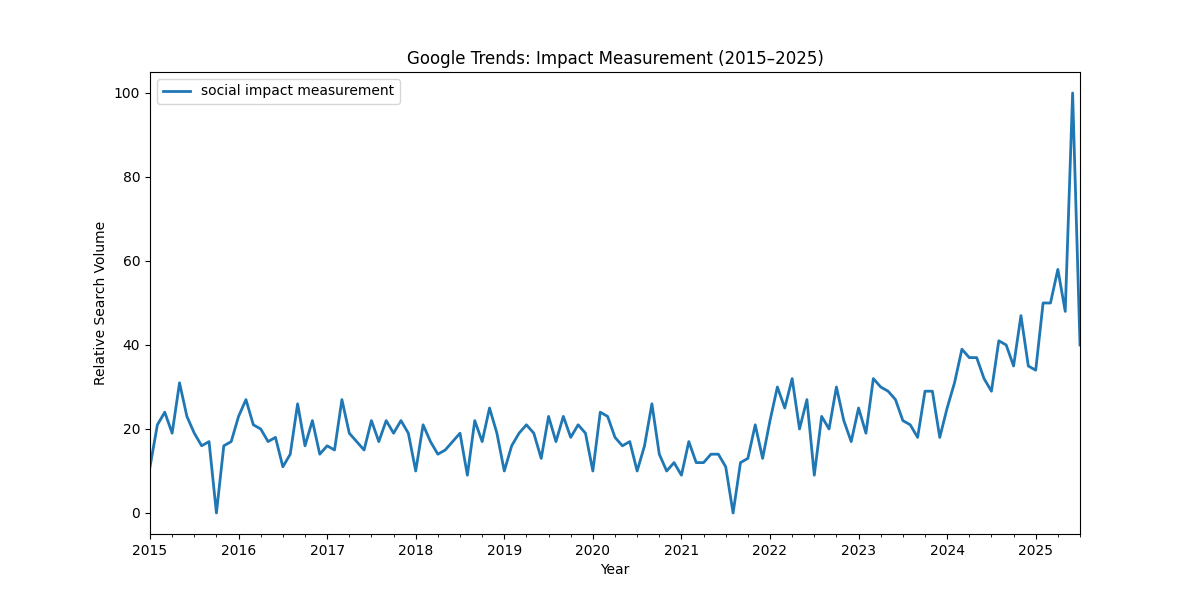
\includegraphics[width = 0.8\textwidth]{../fig/google_trend_impact}
    \caption{Google trend for "impact measurement".}
    \label{fig:trend_impact}
\end{figure}

\section{Public Sector Innovation and Value Creation}\label{sec:public-sector-innovation}
Public sector innovation requires institutions to not only introduce new tools or practices but also foster legitimacy, collaboration, and accountability~\parencite{sun2019algorithmic}.
The OECD has documented challenges and opportunities associated with innovation in government, including an increasing emphasis on public value creation, citizen co-production, and agile experimentation~\parencite{oecd2020publicsector}.

\textcite{wirtz2020public} propose a conceptual model for digital transformation in public services, emphasizing that data-driven approaches can enhance or erode trust depending on their transparency, inclusiveness, and fairness.
The concept of \textbf{public value}—first introduced by Moore (1995) and later expanded—serves as a central reference for evaluating the outcomes of public innovation.
Initiatives such as Project Athena and CityLAB Berlin exemplify stakeholder-driven innovation aligned with public value frameworks.

\section{Artificial Intelligence Methods for Qualitative and Quantitative Data Analysis}\label{sec:ai-methods}
AI has become increasingly prevalent in public governance, ranging from algorithmic decision-making to NLP-based policy analysis.
\textcite{devlin2018bert} introduced BERT, a transformer-based model foundational for text classification, topic modeling, and semantic similarity analysis.
Such methods can be applied to IMM to analyze unstructured stakeholder data, such as survey responses or social media feedback.

\textcite{sun2019algorithmic} caution that AI must be embedded within deliberative governance structures to ensure its use complements rather than replaces human judgment.
Similarly, \textcite{brown2020algorithmic} highlight that while AI can improve monitoring and accountability, it carries risks such as value misalignment, opacity, and exclusion.
In this thesis, AI is employed within the IMM tool \textit{Inluma} to augment human interpretation, particularly in the analysis of complex qualitative narratives.

\section{Synthesis and Gaps}\label{sec:synthesis-gaps}
IMM frameworks, public sector innovation, and AI-supported decision-making offer complementary approaches to tackle complex societal challenges.
However, an integrated framework that unifies these domains is largely absent.
Traditional IMM approaches often rely on structured metrics and overlook unstructured qualitative data~\parencite{epstein_yuthas_2014,fraunhofer_2023}.
Public sector innovation initiatives emphasize stakeholder engagement and legitimacy but underutilize AI to scale qualitative data analysis~\parencite{citylab_2024}.
AI applications, while powerful, often prioritize efficiency over social complexity and normative commitments such as transparency, equity, and public value~\parencite{moore_1995,benington_moore_2011,eu_2024}.

This thesis addresses these gaps by proposing a framework where AI in \textit{Inluma} augments human interpretation, integrates stakeholder input, and aligns with public value principles.
For example, a Hamburg municipality's digital inclusion initiative could be analyzed using NLP tools to identify barriers like affordability, with stakeholders validating results and refining impact metrics.
This framework bridges IMM’s technical limitations and AI’s normative shortcomings, offering an inclusive, transparent, and effective approach to public sector impact measurement.

\begin{figure}[H]
    \centering
    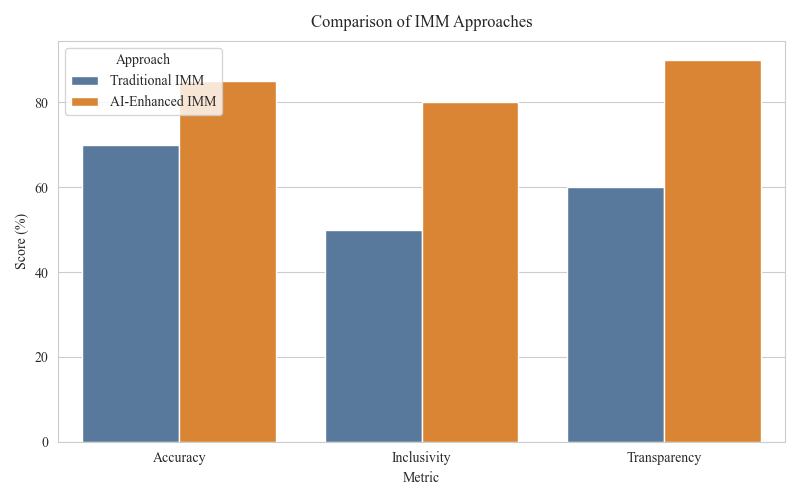
\includegraphics[width=0.8\linewidth]{../fig/imm_comparison}
    \caption{Comparison of IMM frameworks.}
    \label{fig:comparison_imm_fw}
\end{figure}

\section{Conclusion and Research Direction}\label{sec:conclusion}
This chapter has established the theoretical foundation for the thesis, integrating literature on IMM, AI methods, and public sector innovation.
It highlights the research gap that motivates the design, implementation, and evaluation of an AI-supported IMM artefact in \textit{Inluma}.
The following chapter presents the methodology used to develop and assess this framework.